\xiaosi

进入21世纪以来,随着我国工业化过程的加速发展、世界制造业向中国的转移,我国矿产资源的勘探、开发和供给已经成为国民经济持续、稳定、快速发展的重要条件。作为全球制造业大国,与我国巨大的资源消费相比,国内大多数矿产资源的供应远远不能满足国民经济增长的需求。而经过多年的开采,埋藏较浅的易采矿体大多已采完。为了满足国民经济可持续发展的战略需求,人们不得不着手开采深部、赋存条件差的矿体[1]。然而矿业开发一方面促进经济发展和社会进步,另一方面却又可能造成环境破坏。随着国家对环境保护的要求日益严格,矿山如何能够安全高效开采的同时又尽可能减少对环境的影响已成为目前的热点话题。\citep{agrawal2011challenges}\cite{wu2013data}\cite{zhang2016}

\begin{figure}[H]
    \centering
    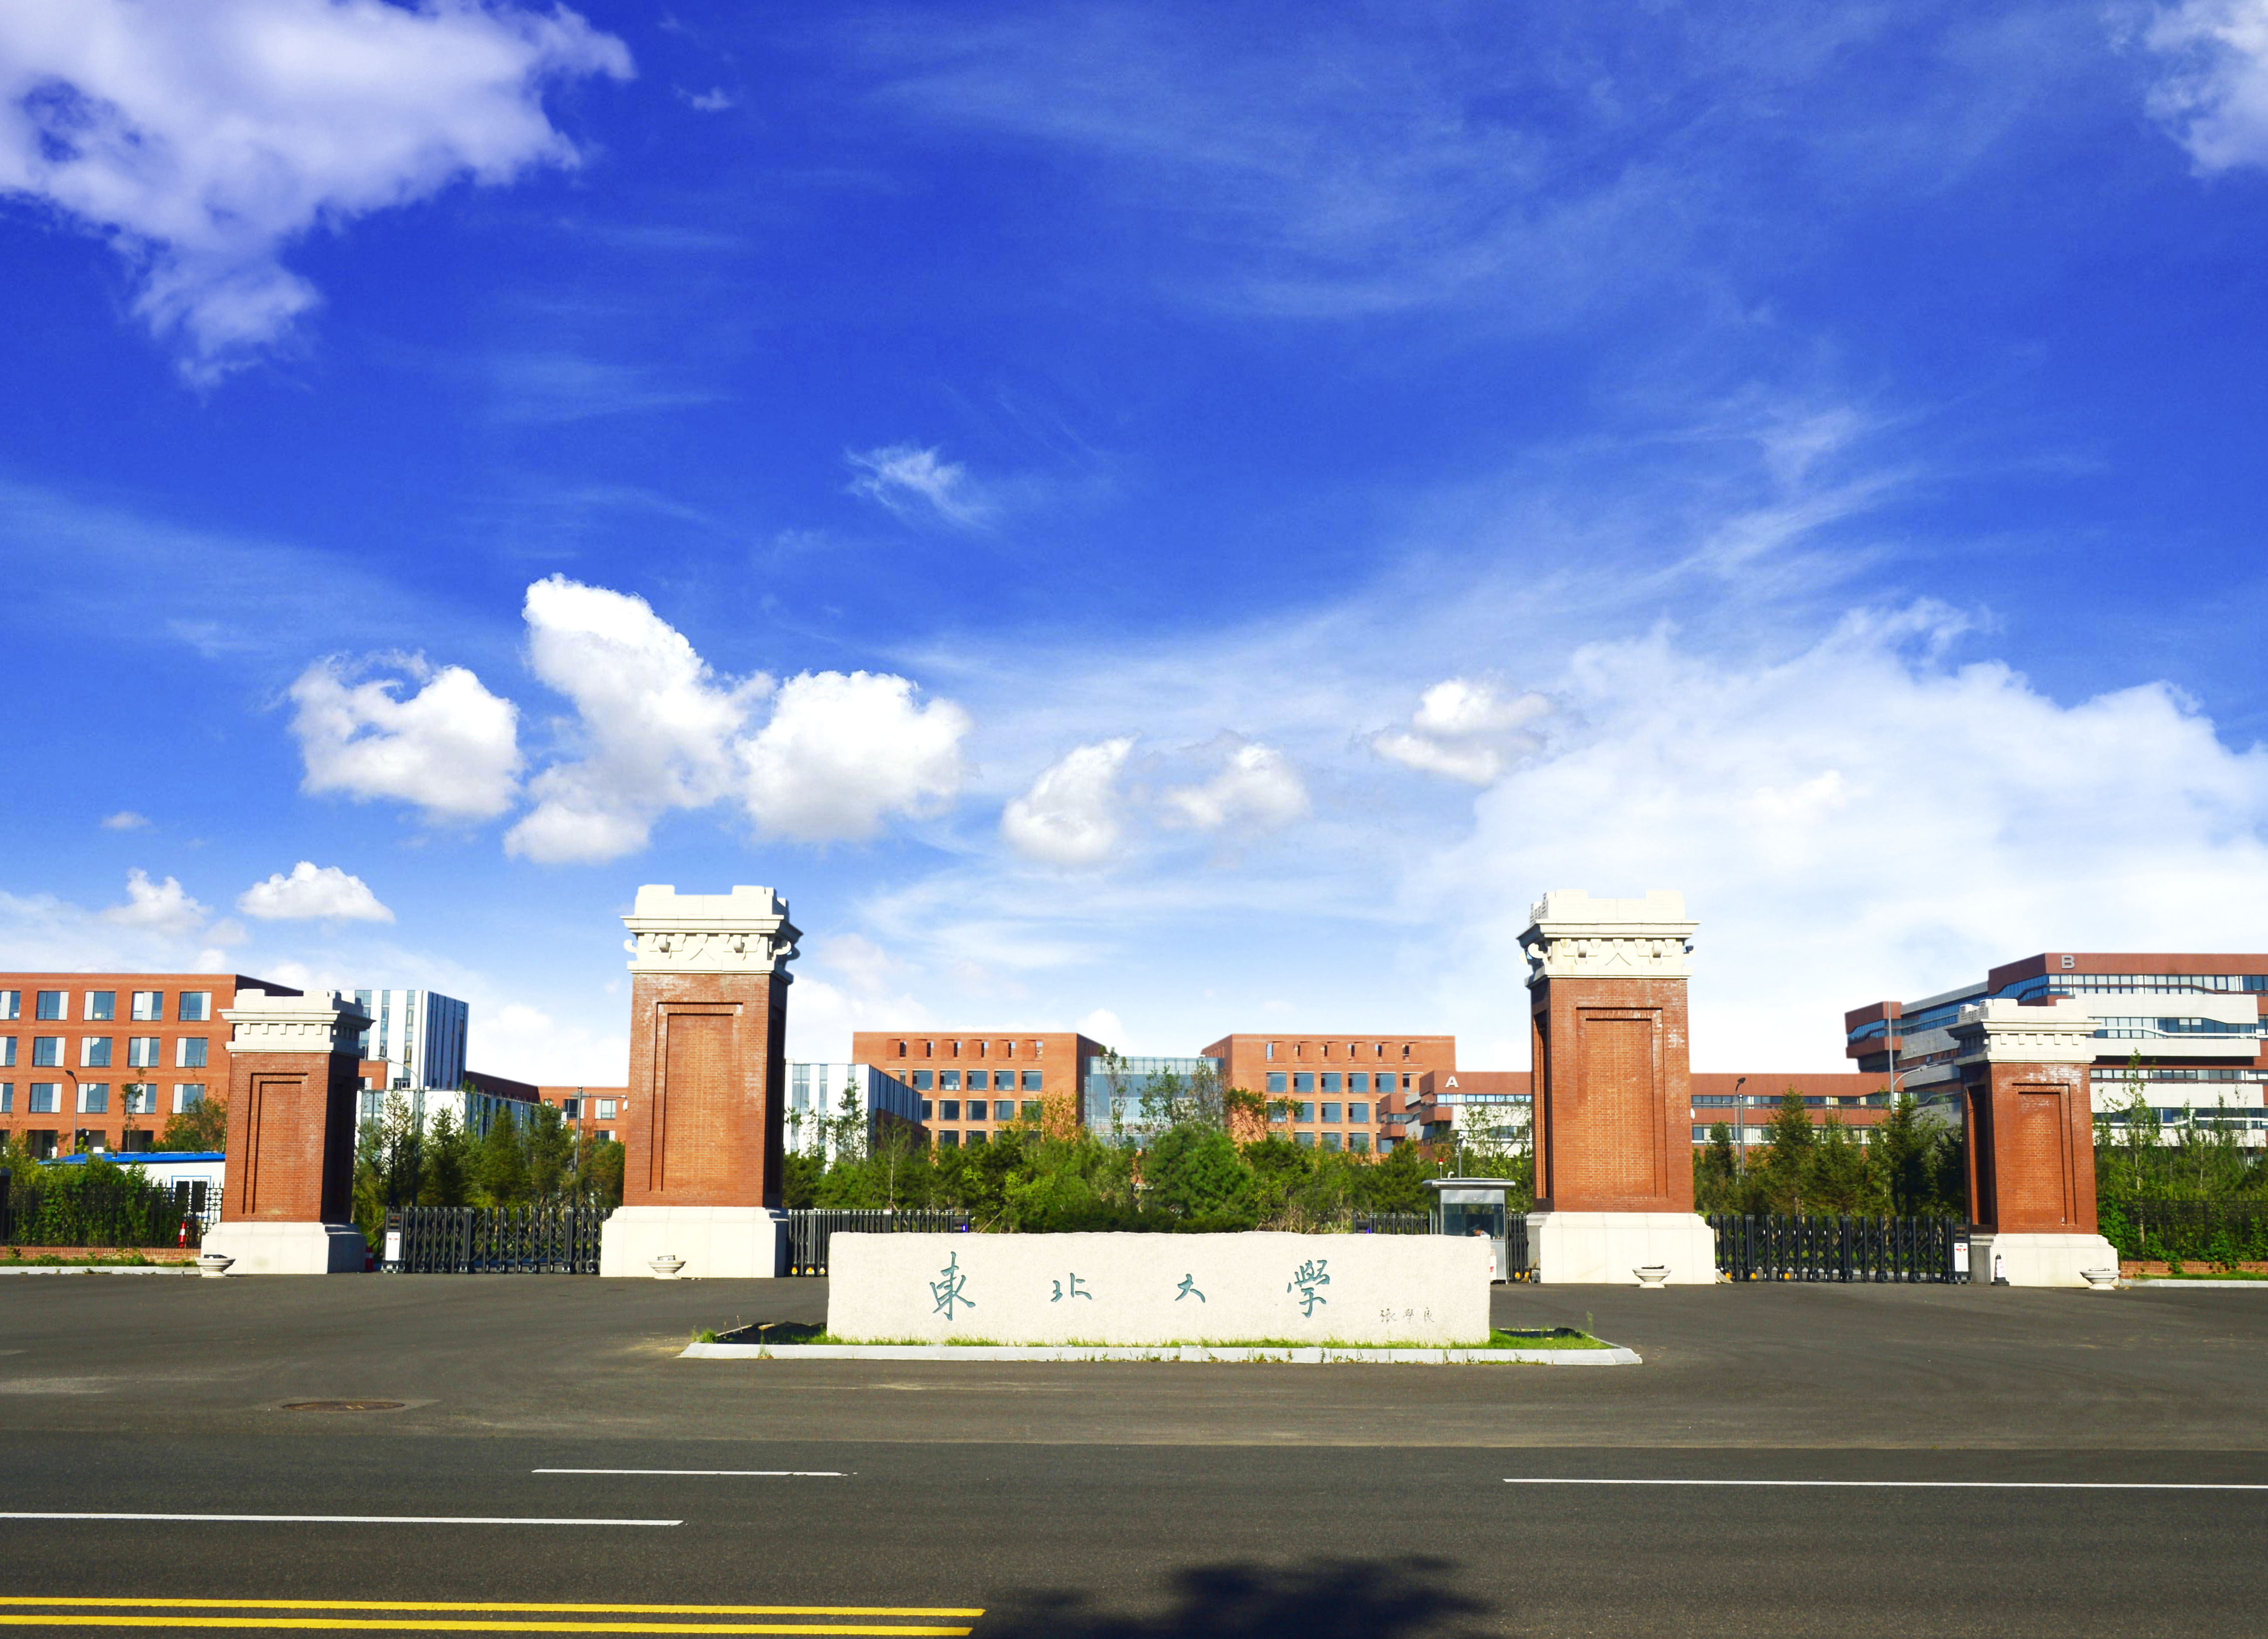
\includegraphics[width=0.8\linewidth]{img/fig1.jpg}
    \caption{一张示例图片}
    \label{fig:figure1}
\end{figure}


